% Created 2021-01-24 Sun 22:50
% Intended LaTeX compiler: pdflatex
\documentclass[11pt]{article}
\usepackage[utf8]{inputenc}
\usepackage[T1]{fontenc}
\usepackage{graphicx}
\usepackage{grffile}
\usepackage{longtable}
\usepackage{wrapfig}
\usepackage{rotating}
\usepackage[normalem]{ulem}
\usepackage{amsmath}
\usepackage{textcomp}
\usepackage{amssymb}
\usepackage{capt-of}
\usepackage{hyperref}
\usepackage{minted}
\hypersetup{colorlinks=true, linkcolor=black, filecolor=red, urlcolor=blue}
\usepackage[turkish]{babel}
\author{Eren Hatırnaz}
\date{27 Ekim 2019}
\title{Yazılım Gündemi - 15\\\medskip
\large 21-27 Ekim 2019}
\hypersetup{
 pdfauthor={Eren Hatırnaz},
 pdftitle={Yazılım Gündemi - 15},
 pdfkeywords={},
 pdfsubject={},
 pdfcreator={Emacs 27.1 (Org mode 9.3)},
 pdflang={Turkish}}
\begin{document}

\maketitle
\tableofcontents \clearpage\shorthandoff{=}

\begin{center}
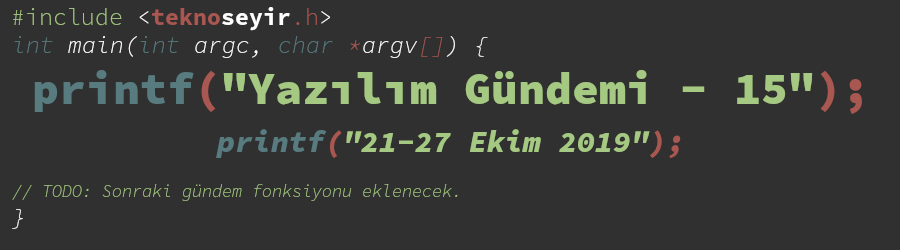
\includegraphics[width=.9\linewidth]{gorseller/yazilim-gundemi-banner.png}
\end{center}

\begin{center}
\href{../14/yazilim-gundemi-14.pdf}{< Önceki Gündem} | \textbf{21-27 Ekim 2019} | \href{../16/yazilim-gundemi-16.pdf}{Sonraki Gündem >}

\href{https://teknoseyir.com/blog/yazilim-gundemi-15-21-27-ekim-2019}{TeknoSeyir'de Oku}
\end{center}

\section{Yeni bir önbellek zehirleme açığı ortaya çıktı: \href{https://cpdos.org/}{CPDoS}}
\label{sec:org98e25e3}
Gün geçmiyor ki yeni bir güvenlik açığı daha ortaya çıkmasın. Alman siber
güvenlik araştırmacıları, bu hafta yayınladıkları "\href{https://cpdos.org/paper/Your\_Cache\_Has\_Fallen\_\_Cache\_Poisoned\_Denial\_of\_Service\_Attack\_\_Preprint\_.pdf}{Your Cache Has Fallen:
Cache-Poisoned Denial-of-Service Attack}" başlıklı makaleleriyle yeni bir açığı
ortaya çıkardı. Üstelik bu açıktan sektörde sıkça kullanılan Amazon CloudFront,
Cloudflare, Akamai gibi CDN (Content Delivery Network) hizmetlerini de
etkiliyor.

\begin{figure}[htbp]
\centering
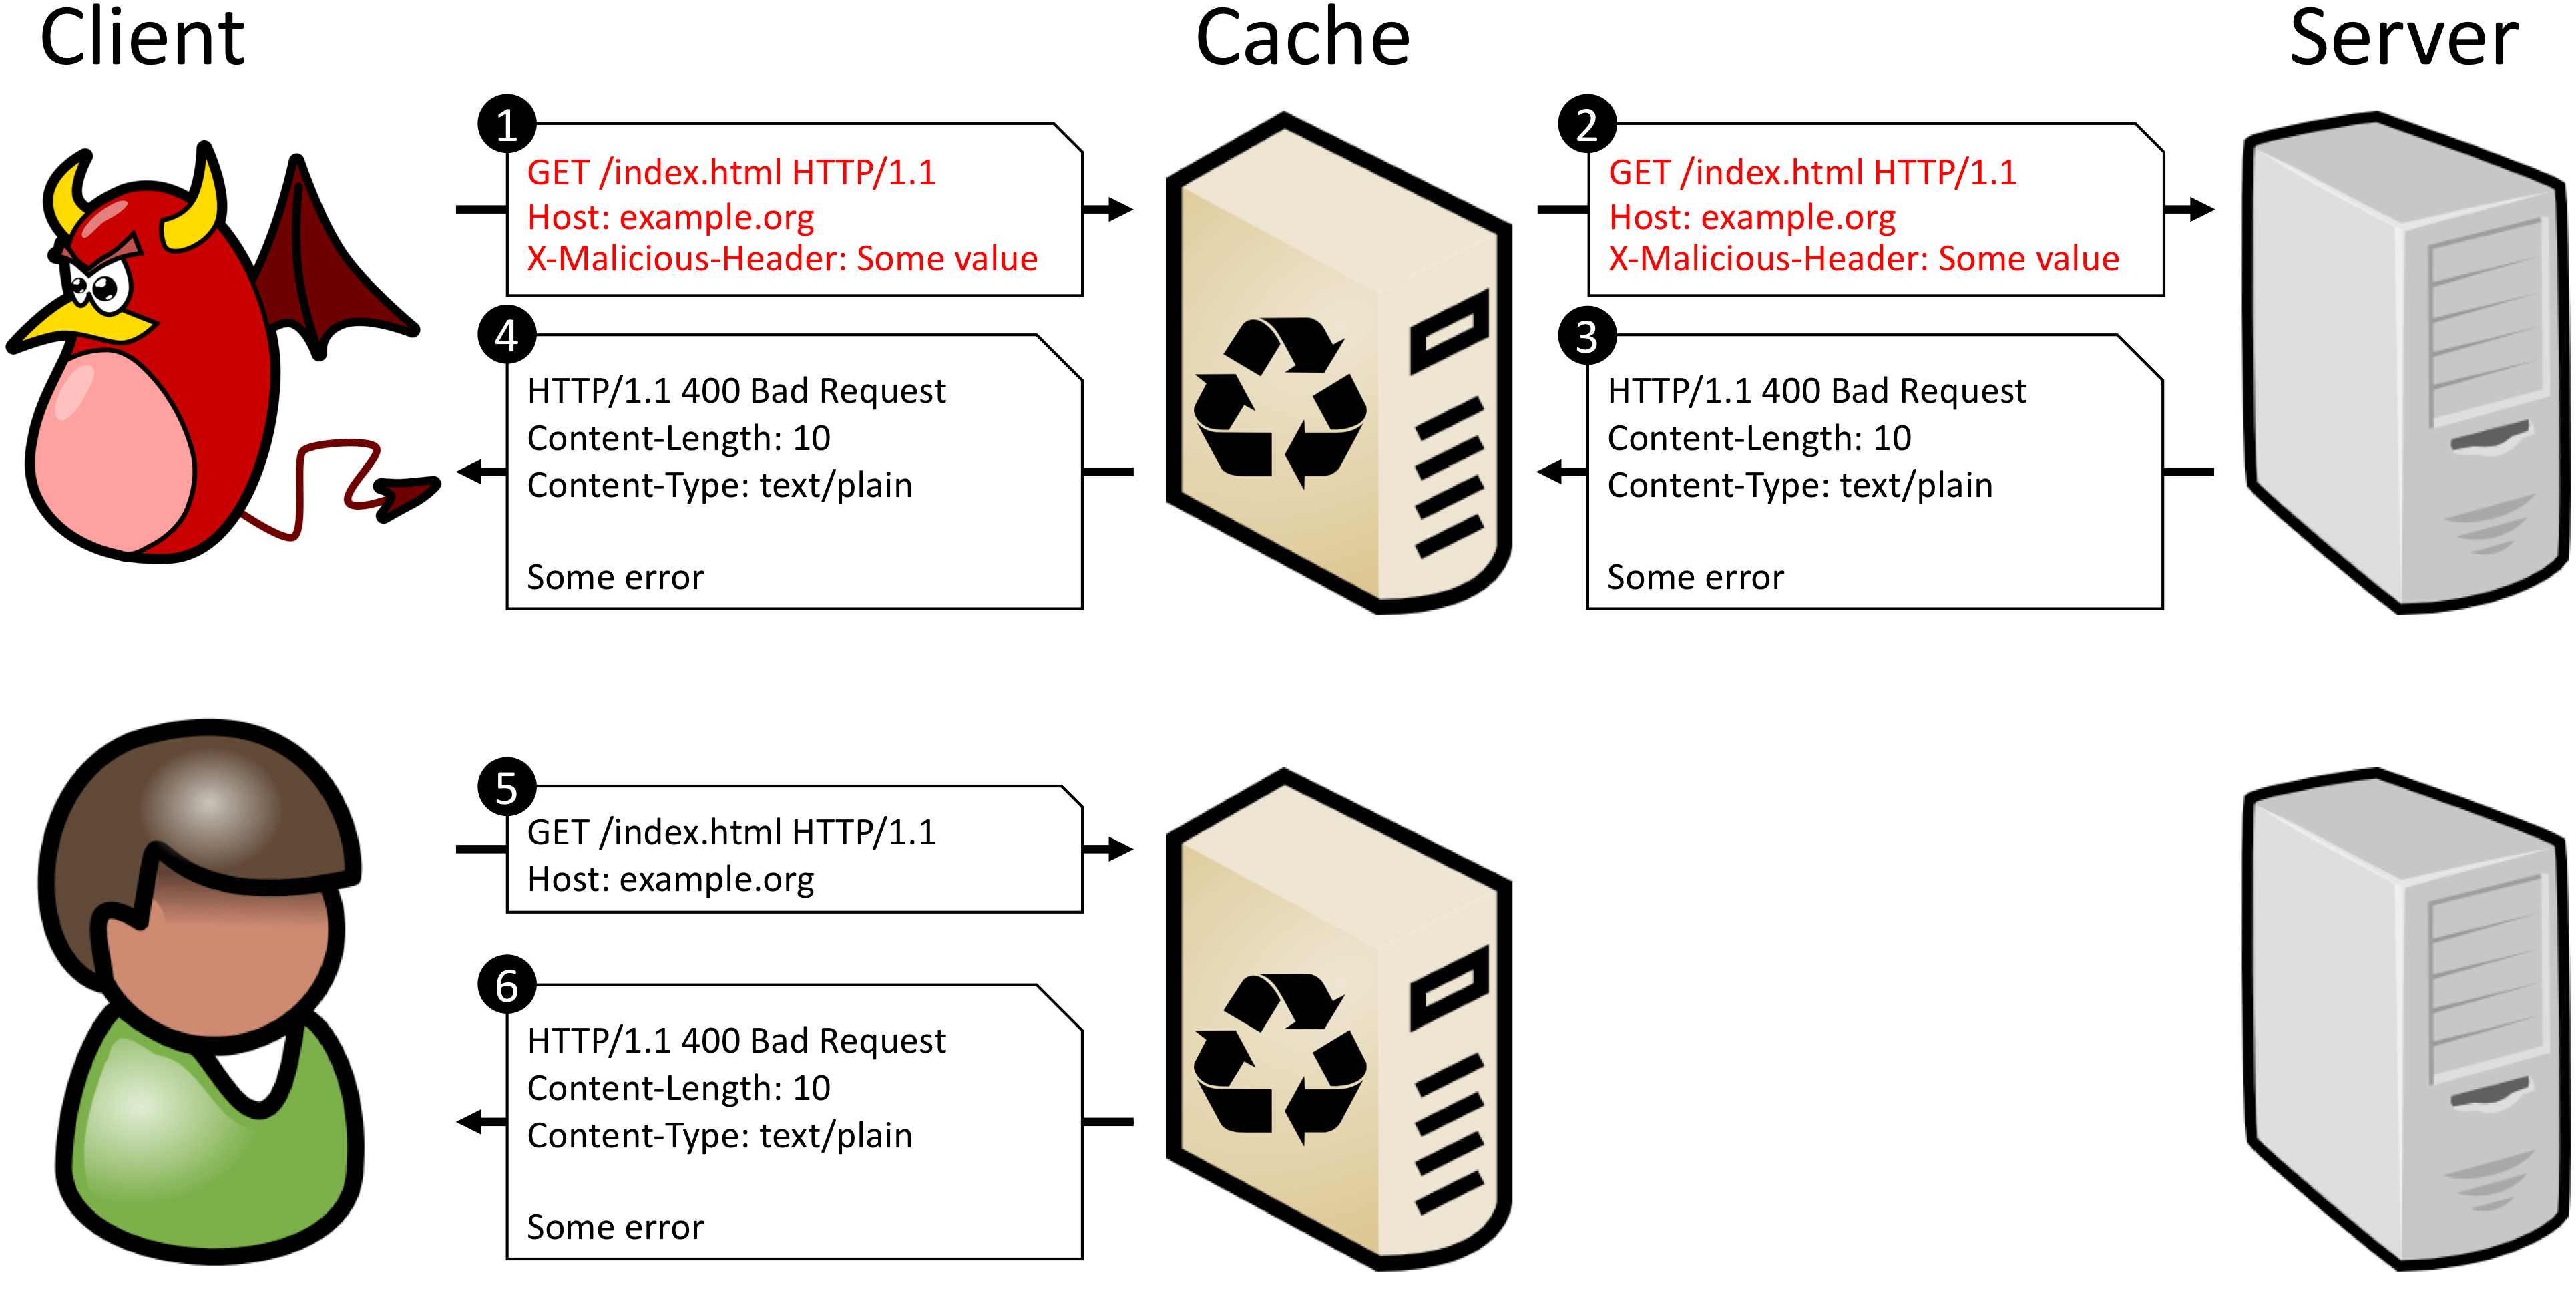
\includegraphics[width=.9\linewidth]{gorseller/CPDoS.png}
\caption{CPDoS Açığı}
\end{figure}

Görselden yola çıkarak açığı açıklamak gerekirse:
\begin{enumerate}
\item Saldırgan sitenin kabul etmediği bir HTTP Header bilgisiyle GET isteği
yapıyor. (Örn: \texttt{X-Zararli-Baslik: Deneme})
\item Önbellek sunucusu böyle bir isteği daha önce hafızasında tutmadığı için
isteği gerçek sunucuya gönderiyor.
\item Gerçek sunucu da böyle bir HTTP Header bilgisini kabul etmediği için
önbellek sunucusuna hata mesajı gönderiyor.
\item Önbellek sunucusu, gerçek sunucudan aldığı sayfayı aynen saldırgana
gönderiyor.
\item Normal kullanıcı siteye normal bir GET isteği gönderiyor.
\item Önbellek sunucusu kullanıcıya yine hafızasındaki hata sayfasını
gönderiyor.
\end{enumerate}

Aslında bu açığın 3 tane de alt türü mevcut. Bunlar da şu şekilde:
\begin{itemize}
\item \textbf{HTTP Header Oversize (HHO):} HTTP isteğinin boyutunu aşırı yükselterek
siteyi hata vermeye zorlama.
\item \textbf{HTTP Meta Character (HMC):} HTTP isteğine zararlı karakter (\texttt{\textbackslash{}n},
\texttt{\textbackslash{}r}, \texttt{\textbackslash{}a} gibi) ekleyerek siteyi hata vermeye zorlama.
\item \textbf{HTTP Method Override (HMO):} Sitenin kabul etmediği HTTP methodları
(DELETE gibi) göndererek siteyi hata vermeye zorlama.
\end{itemize}

Açığın nasıl kullanıldığını gösteren bir videoyu \href{https://www.youtube.com/watch?v=c4-1UaEEwI8}{bu adresten} izleyebilirsiniz.
Açıktan etkilenen web sunucu ve CDN hizmetlerinin listesi ise bu şekilde:

\begin{figure}[htbp]
\centering
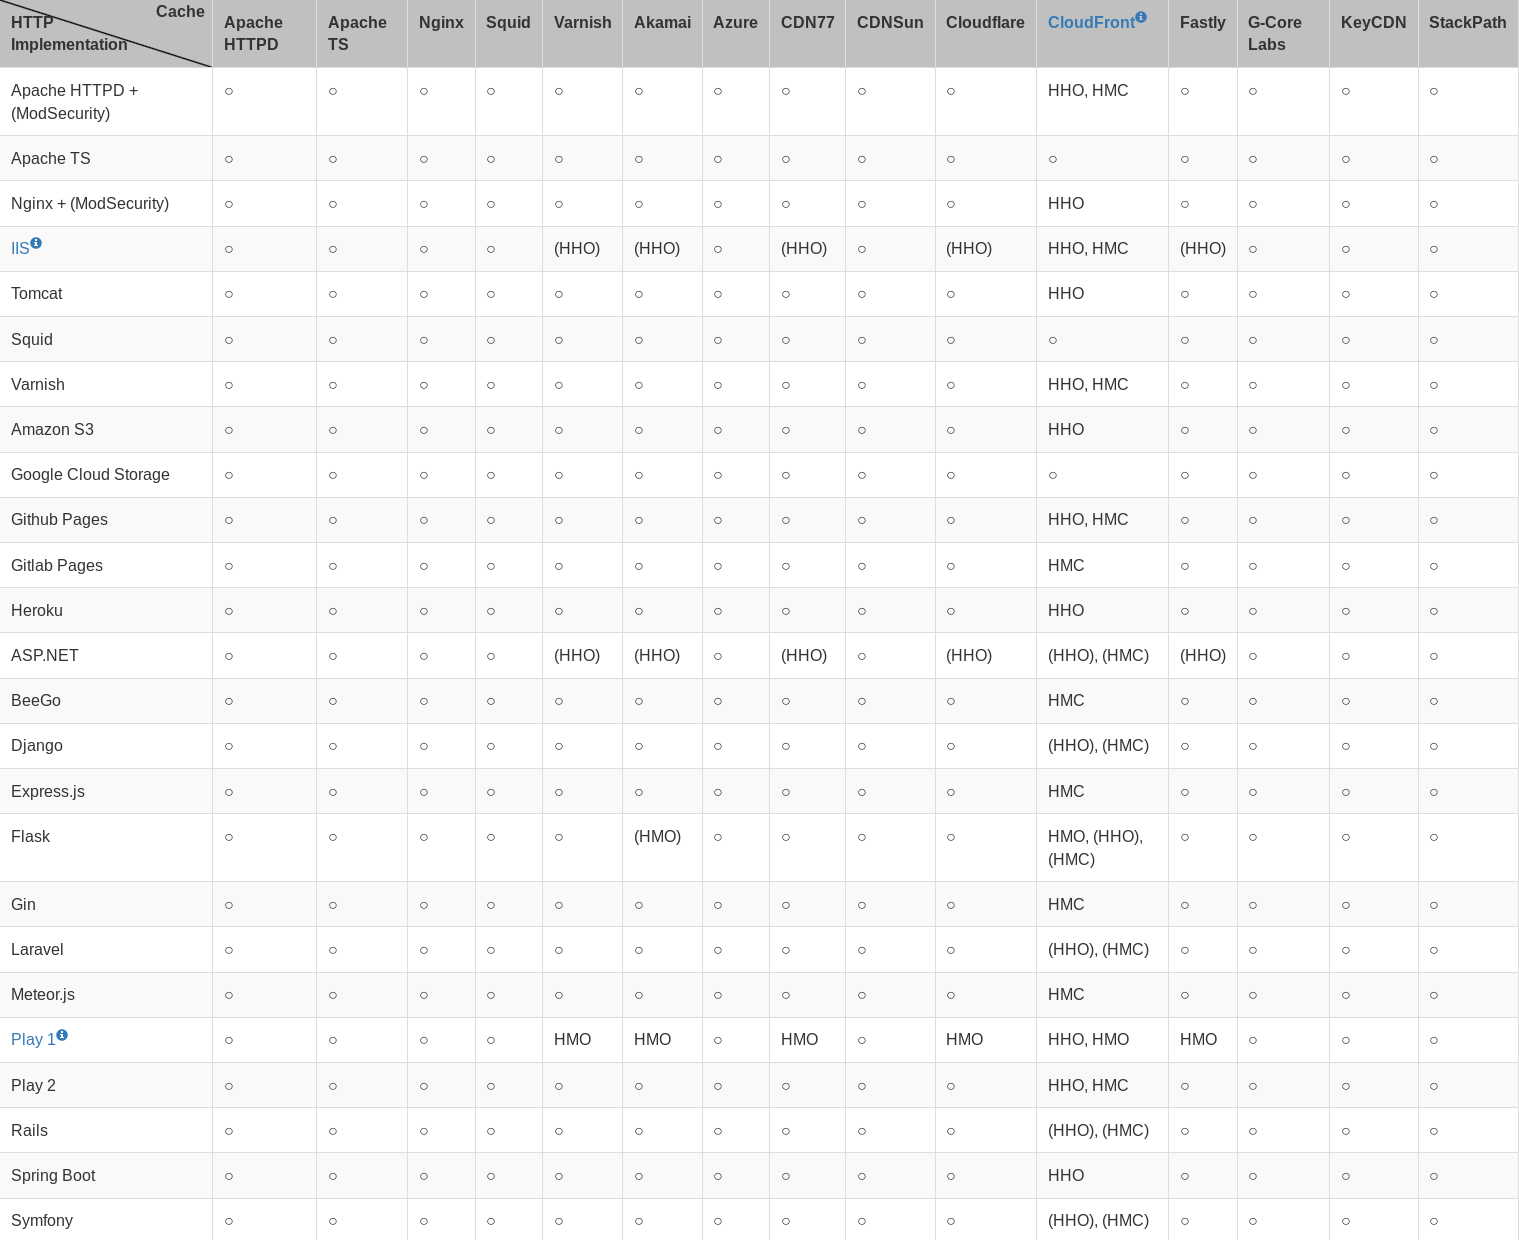
\includegraphics[width=.9\linewidth]{gorseller/cpdos-etkileri.png}
\caption{Yukarıdaki açık türlerinin kısaltmaları bu tablodaki bir hücrede varsa o sistemde açık var demektir}
\end{figure}

Yalnız tabii ki de etik kurallar gereği bulunan açık önce etkilenebilecek
firmalarla paylaşıldığı için çoğu web sunucusu ve CDN hizmeti sağlayan firmalar
açıkları gidermiş durumda. Yani korkacak bir şey yok gibi gözüküyor.

Daha detaylı bilgi için konu başlığına eklediğim bağlantıdaki sayfayı ziyaret
edebilirsiniz.
\section{PHP-FPM'deki hata saldırganların uzaktan \href{https://thehackernews.com/2019/10/nginx-php-fpm-hacking.html}{kod çalıştırmasına olanak sağlıyor}}
\label{sec:orgebb3404}
\href{https://php-fpm.org/}{PHP-FPM (FastCGI Process Manager)}, normal PHP'deki FastCGI implementasyonuna
alternatif daha gelişmiş ve yüksel verimlilik sunan bir işleyici. Fakat bu
projedeki bir bellek hatası, diğer birkaç sorunla daha birleşince
saldırganların sunucuda zararlı kod çalıştırabileceği bir güvenlik zafiyeti
haline geliyor. Her ne kadar bu açığı meydana getiren koşulların bir araya
gelmesi zor gözükse de güvenlik açığı sonuçta, ihmal etmeye gelmez.

Wallarm isimli şirkette güvenlik araştırmacısı olarak çalışan Andrew Danau
tarafından \href{https://lab.wallarm.com/php-remote-code-execution-0-day-discovered-in-real-world-ctf-exercise/}{ortaya çıkarılan} bu açığı exploit edenler ise Omar Ganiev ve Emil
Lerner.

Güvenlik zafiyetinin oluşabilmesi için gerekli koşullar ise şu şekilde:
\begin{itemize}
\item NGINX web sunucusunun PHP-FPM ile çalışması için ayarlanmış olması,
\item \texttt{fastcgi\_split\_path\_info} direktifinde \textbf{\^{}} ile başlayan ve \textbf{\$} ile biten
bir regex ifadesinin tanımlı olması
\item \texttt{PATH\_INFO} değişkeninin \texttt{fastcgi\_param} direktifi ile tanımlanması,
\item ve istenen dosyanın olup olmadığını kontrol eden herhangi bir ayarın
olmaması,
\end{itemize}
NGINX'de şöyle ayarlar varsa:
\begin{minted}[breaklines=true,breakanywhere=true,frame=lines, linenos, label=NGINX, labelposition=topline]{nginx}
location ~ [^/]\.php(/|$) {
  # ...
  fastcgi_split_path_info ^(.+?\.php)(/.*)$;
  fastcgi_param PATH_INFO       $fastcgi_path_info;
  fastcgi_pass   php:9000;
  # ...
}
\end{minted}
güvenlik zafiyeti de oluşmuş oluyor. Saldırgan da regex ifadesini bir şekilde
maniple ederek bu bellek hatasını tetikliyor ve URL üzerinden istediği
komutları çalıştırabilir hale geliyor.

\begin{figure}[htbp]
\centering
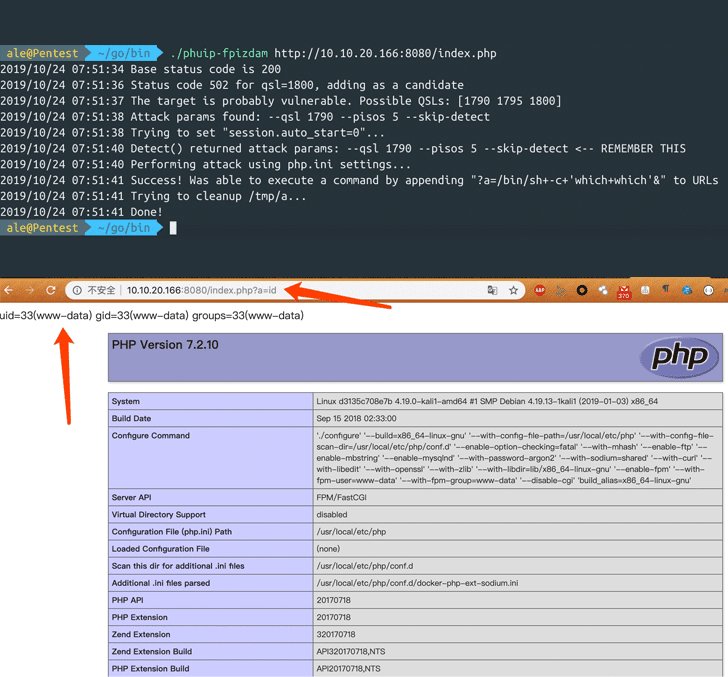
\includegraphics[width=.9\linewidth]{gorseller/php-fpm-acik.png}
\caption{Görselde kullanılan exploit \href{https://github.com/neex/phuip-fpizdam}{bu adreste} yayınlanmış}
\end{figure}

PHP 7.3.11 ve PHP 7.2.24 sürümlerinde bu açıklar giderilmiş. Siz de
sunucularınızdaki NGINX ayarlarınızı kontrol edin ve ilgili PHP
güncellemelerini yapmayı ihmal etmeyin.
\newpage
\section{GitLab, hizmetlerine telemetri servisi eklemek istedi fakat vazgeçti}
\label{sec:orge6d20a4}
GitLab geçtiğimiz haftalarda yayınladığı bir \href{https://about.gitlab.com/blog/2019/10/10/update-free-software-and-telemetry/}{blog yazısıyla} kullanıcılara daha
iyi hizmet verebilmek için GitLab.com ve ilgili servislerine telemetri (sayfayı
ziyaret eden kullanıcıların davranışlarıyla ilgili raporlar hazırlayan
servislere verilen isim) ekleyeceğini duyurmuştu. GitLab'ın bu girişimi, her ne
kadar, "Eğer tarayıcınızın Do Not Track (DNT- Beni takip etme) ayarını
kullanıyorsanız buna saygı göstereceğiz" ve "GitLab Community Edition'da böyle
bir şey olmayacak" deseler bile geliştirici toplulukları tarafından hiç hoş
karşılanmadı ve \href{https://news.ycombinator.com/item?id=21343761}{HackerNews} ve \href{https://www.reddit.com/r/programming/comments/dm72oa/gitlab\_mandating\_thirdparty\_telemetry\_locks\_out}{Reddit} gibi platformlarda tartışmalara yol açtı.
Bunun üzerine GitLab'da ilgili blog yazısına bir güncelleme notu ekleyerek, bu
değişikliklerden vazgeçtiklerini ve üzerine \href{https://gitlab.com/gitlab-com/www-gitlab-com/issues/5672}{biraz daha çalışacaklarını}
duyurdular.

Bu konu hakkında siz ne düşünüyorsunuz? Hem bir geliştirici olarak hem de bir
kullanıcı olarak telemetri servisleriyle ilgili genel görüşünüz nedir? Yorumlar
kısmında konuşalım.
\section{TypeScript \href{https://devblogs.microsoft.com/typescript/announcing-typescript-3-7-rc/}{3.7 RC sürümü duyuruldu}}
\label{sec:org4f8c36f}
Microsoft tarafından geliştirilen tip destekli JavaScript yazmayı sağlayan
TypeScript dilinin bu hafta 3.7 RC sürümü duyuruldu. Daha \href{https://github.com/microsoft/TypeScript/issues/33352}{önce yayınlanan
planda dokümanı}nda da belirtilen tarihten 2 gün sonra gerçekleşmiş olsa da her
şey yolunda gözüküyor. TypeScript 3.7 ile gelecek iki özelliğe daha önceki
gündem yazılarında değinmiştik (bkz: \href{../09/yazilim-gundemi-09.pdf}{Yazılım Gündemi - 9}). O yazıdaki
özellikler haricinde yeni eklenen bir özelliğe daha göz atalım demek isterdim
fakat ilgili blog yazısındaki "\emph{Assertion Functions}" bölümünü okumama rağmen
tam olarak anlayamadım, sanırım bunda uzun zamandır JavaScript yazmıyor
olmamın da payı var.

Daha detaylı bilgi ve eklenen özelliklerle ilgili konu başlığına eklediğim
bağlantıya tıklayabilirsiniz.
\section{Turkcell'in, Firefox Preview lisansını \href{https://twitter.com/FirefoxPreview/status/1187461728709173254?s=20}{ihlal ettiği ortaya çıktı}}
\label{sec:orgdbe593b}
Turkcell'in geliştirdiği "yerli arama motoru" Yaani'nin, mobil cihazlar için
geliştirdiği tarayıcısı, Firefox Preview'den forklanarak oluşturulmuş bir
tarayıcı. Bunda bir sıkıntı yok. Firefox zaten açık kaynak kodlu ve özgür
lisanslı bir uygulama, nitekim Tor Browser da Firefox'dan forklanmış. Fakat
sorun Turkcell, Firefox Preview'in lisansı olan \href{https://www.mozilla.org/en-US/MPL/2.0/}{Mozilla Public License 2.0}'ı
ihlal etmesi. Yaani tarayıcısı açılırken bir kullanım sözleşmesi gösteriyor ve
burada da MPL 2.0 lisansı listelenmiş fakat bu lisansın bir şartı olan kodların
aynı lisans ile paylaşılması maddesi ihlal edilmiş (Madde 3.2). Turkcell, Yaani
mobil uygulamasının kodlarını henüz hiçbir yerde paylaşmış değil. Konu Türkiye
basınında hiç yer almadı, dolayısıyla Turkcell konuyla ilgili bir cevap da
yayınlamış değil.

\begin{figure}[htbp]
\centering
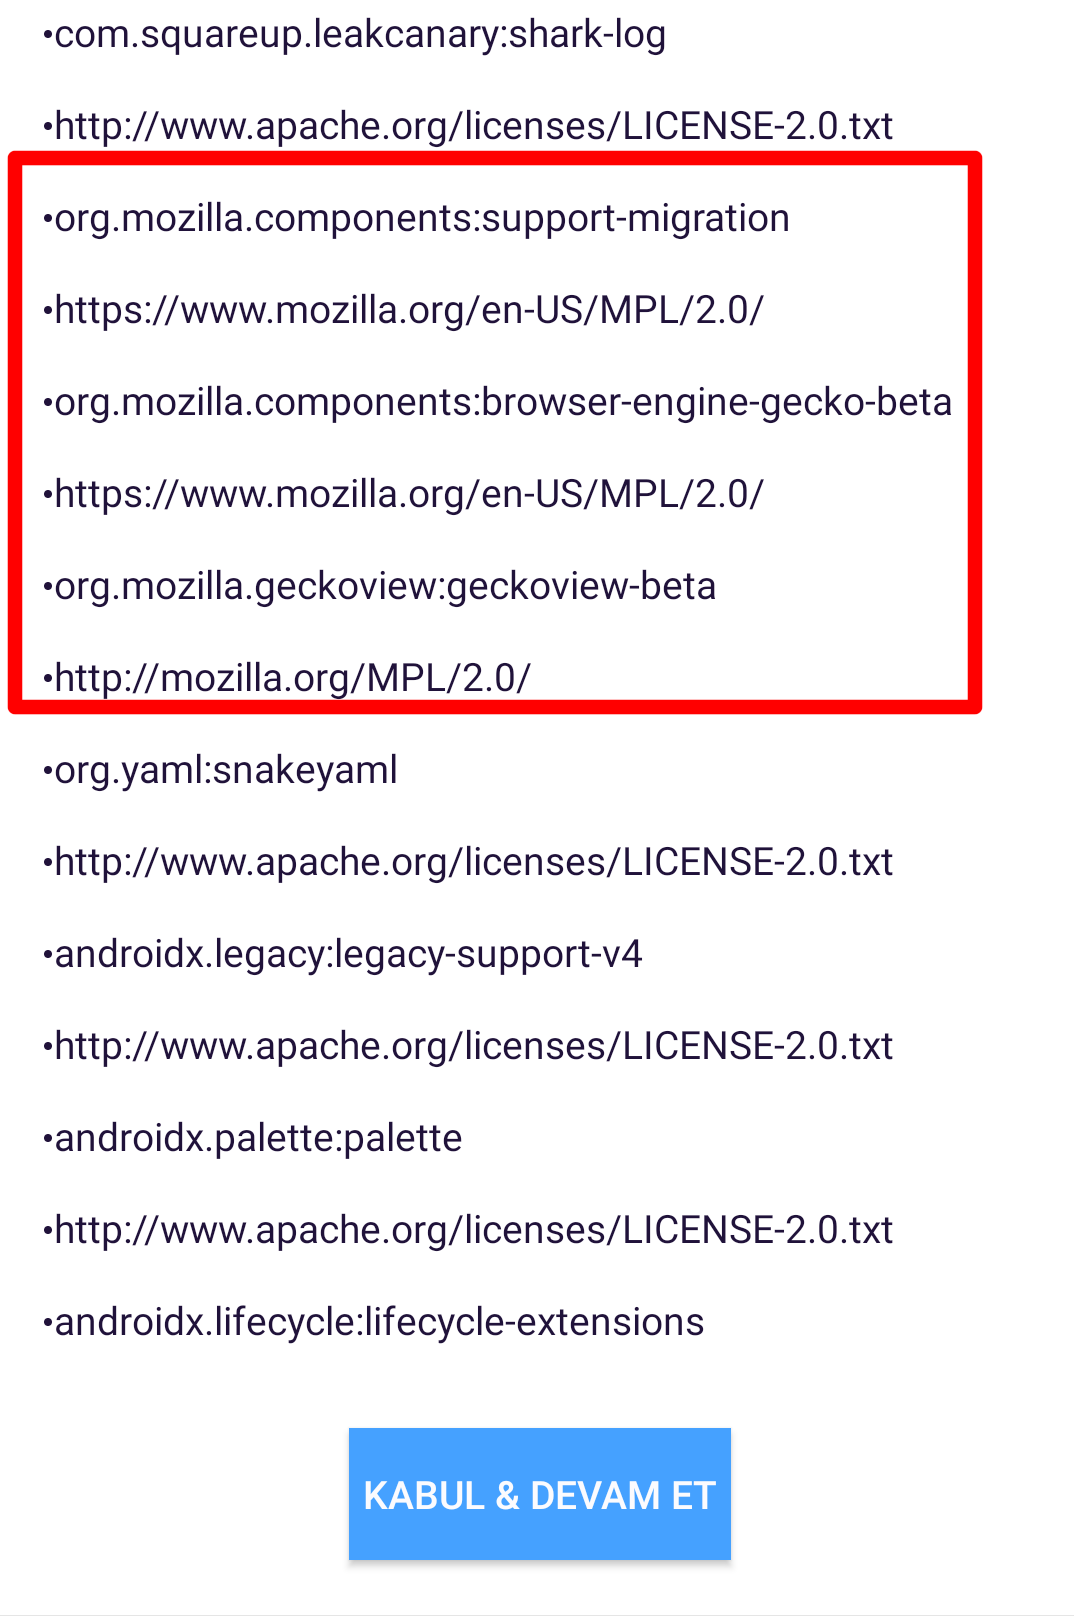
\includegraphics[height=10cm]{gorseller/turkcell-mpl-ihlal.png}
\caption{Turkcell Yaani uygulamasının kullanım sözleşmesinde MPL 2.0 lisansı listelenmiş.}
\end{figure}

Konuyla ilgili siz ne düşünüyorsunuz diyeceğim ama pek şaşırdığınızı
düşünmüyorum bu habere. Ben de şaşırmadım. Daha açık kaynak kullandığımız
kodların lisanslarına bile saygı duymuyorken, Türkiye'den bir Google çıkmasını
beklemek saçma olur diye düşünüyorum.
\section{Firefox 70 ile gelen \href{https://hacks.mozilla.org/2019/10/firefox-70-a-bountiful-release-for-all/}{yeni özellikler}}
\label{sec:orgc0db7d0}
Bu hafta Firefox tarayıcısının 70 numaralı sürümü yayınlandı. Normal
kullanıcıları ilgilendiren özelliklerin bir kısmını \href{https://teknoseyir.com/durum/1162388}{şuradaki paylaşımım}da
özetlemiştim. Şimdi de biz geliştiricileri ilgilendiren birkaç değişikliğe
bakalım:

\subsection{[CSS] Altı çizgili yazılar için yeni seçenekler}
\label{sec:org9a4d115}
Artık altı çizgili yazılarımızı daha da özelleştirebileceğiz. Şöyle ki:
\begin{itemize}
\item \textbf{\href{https://developer.mozilla.org/en-US/docs/Web/CSS/text-decoration-thickness}{text-decoration-thickness}} ile alt çizginin boyutunu değiştirebiliyoruz,
\item \textbf{\href{https://developer.mozilla.org/en-US/docs/Web/CSS/text-underline-offset}{text-underline-offset}} ile alt çizginin konumunu değiştirebiliyoruz,
\item \textbf{\href{https://developer.mozilla.org/en-US/docs/Web/CSS/text-decoration-skip-ink}{text-decoration-skip-ink}} ile de alt çizginin, harflerin kuyruklarından
geçerken çizilmemesini sağlayabilirsiniz. Bu özellik artık varsayılan
olarak \texttt{auto} olacak.
\end{itemize}
Böyle kuru kuru olmadı gelin bir örnek yapalım:
\begin{minted}[breaklines=true,breakanywhere=true,frame=lines, linenos, label=HTML, labelposition=topline]{html}
<style>
  h1 {
  text-decoration: underline red;
  text-decoration-thickness: 3px;
  text-underline-offset: 6px;
  }
</style>

<h1>selam teknoseyir <br/> bu firefox'un yeni css özelliği</h1>
\end{minted}

ve işte sonuç:

\begin{center}
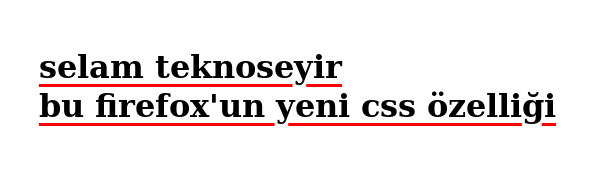
\includegraphics[width=.9\linewidth]{gorseller/firefox-yeni-css.png}
\end{center}
\subsection{[JS] \href{https://developer.mozilla.org/en-US/docs/Web/JavaScript/Reference/Lexical\_grammar\#Numeric\_separators}{Numeric Separators}}
\label{sec:orge3c5143}
Türkçe'ye sanırım numara ayırıcılar olarak çevirebiliriz bu özelliği. Bu yeni
özellik sayesinde artık JavaScript'de sayı değişkeni tanımlarken daha kolay
okuyabilmek için bu şekilde sayıların basamaklarını ayırabileceğiz:
\begin{minted}[breaklines=true,breakanywhere=true,frame=lines, linenos, label=JavaScript, labelposition=topline]{javascript}
let sayi1=1_000_000;
console.log(sayi1); // çıktı: 1000000
\end{minted}
Öyle çok olmazsa olmaz bir özellik değil ama yine de faydalı.

İncelediğim iki özelliğin de diğer tarayıcılardaki desteklenme durumlarını
kontrol etmek için eklediğim bağlantılardaki "\emph{Browser compatibility}"
bölümüne göz atabilirsiniz. Ayrıca diğer eklenen özellikler için de konu
başlığına eklediğim bağlantıya tıklayabilirsiniz.
\section{Chrome 80 sürümünde \texttt{SameSite=None; Secure} \href{https://blog.chromium.org/2019/10/developers-get-ready-for-new.html?m=1}{özelliği gelecek}}
\label{sec:orgf0a37c2}
Çerezler (cookies) hem güvenliklerinin sağlanması açısından hem de
yönetimlerinin zor olması açısından geliştiricileri uğraştırmalarıyla ünlü
yapılardır. Özellikle de \href{https://cheatsheetseries.owasp.org/cheatsheets/Cross-Site\_Request\_Forgery\_Prevention\_Cheat\_Sheet.html}{Cross-Site Request Forgery (CSRF)} olarak bilinen
güvenlik zafiyeti, bir dönem her geliştiricinin korkulu rüyasıydı. Neyse ki
tarayıcılardaki cookie özelliklerinin gelişmesiyle ve geliştiricilerin de
bilinçlenmesiyle o günler geride kaldı.

Chromium takımı bu hafta yayınladıkları blog yazısı ile biz geliştiricileri
\texttt{SameSite=None; Secure} özelliğine hazır olmaya çağırıyor fakat bu özelliğin
neleri değiştirdiğinizi anlamak için önce Cross-Site ve Same-Site kavramlarına
bakmamız gerek.

Her cookie bir domain ile ilişkilendirilmiştir. Eğer bu domain ile tarayıcının
adres çubuğundaki domain farklı ise bu Cross-Site Cookie; aynı ise Same-Site
Cookie ismini alıyor. Cross-Site Cookie'ler ziyaret ettiğimiz bir çok web
sitesinin üçüncü parti olarak sitesine eklediği hizmetlerden (reklam,
istatistik vb.) gelebilir. Same-Site cookie'ler ise genellikle kullanıcıları
siteye giriş yapılmış tutmak (beni hatırla seçeneği) için kullanılır. Doğal
olarak bu Same-Site cookie'lere dışarıdan erişilmesini istemiyoruz. Bu noktada
kullanabileceğimiz iki ayar (\texttt{SameSite=Lax} ve \texttt{SameSite=Strict}) hali hazırda
zaten mevcut fakat artık Chrome aksi belirtilmediği sürece tüm cookie'leri
dışarıdan erişilmesi istenmeyen, yani Same-Site olarak değerlendirecek. Aksini
belirtmek için, yani cookie'yi Cross-Site yapmak için de \texttt{SameSite=None;
	Secure} özelliğini kullanmamız gerekecek ve Cross-Site cookie kullanacak
sitelerin de artık HTTPS olmaları zorunlu olacak. Bu elbette cross-site
güvenlik tehditlerini tamamen ortadan kaldırmayacak ama ağ üzerinden yapılacak
manipülasyonların büyük oranda önüne geçmiş olacak.

2020 Şubat ayında yayınlanması planan Chrome 80 sürümüyle hayatımıza girecek
olan bu değişikliğe hazır olmak için yapılması gerekenleri şu şekilde sıralamış
Google:
\begin{itemize}
\item Bazı dillerde ya da kütüphaneler henüz \texttt{None} değerini desteklemiyor
olabilir. Böyle bir durumda cookie header bilgisine kendiniz eklemeniz
gerekecek. Bazı dil ve kütüphanelerde bunun nasıl yapılacağını anlatan
şöyle bir depo hazırlamış Google:
\url{https://github.com/GoogleChromeLabs/samesite-examples}
\item Bazı tarayıcılar ya da tarayıcıların eski versiyonları \texttt{None} değerini
desteklemiyor olabilir. Uyumsuz istemciler listesine buradan
bakabilirsiniz:
\url{https://www.chromium.org/updates/same-site/incompatible-clients}
\item Diğerleri için konu başlığına eklediğim bağlantıdaki blog yazısının "\emph{How
to Prepare; Known Complexities}" bölümüne bakabilirsiniz.
\end{itemize}

Ayrıca bu davranışı test etmek için Chrome 76 ve yukarısındaki sürümler için
\emph{chrome://flags} adresinden "\emph{SameSite by default cookies}" ve "\emph{Cookies
without SameSite must be secure}" ayarlarını açabilirsiniz.

Same-Site Cookie'lerle ilgili daha detaylı bilgi için \href{https://web.dev/samesite-cookies-explained/}{bu adresi} ziyaret
edebilirsiniz.
\section{Yeni bir Qt aracı duyuruldu: \href{https://www.qt.io/blog/web-based-qt-design-viewer}{Qt Design Viewer}}
\label{sec:orga942fd3}
\href{https://doc.qt.io/qt-5/wasm.html}{Qt for WebAssembly} üzerinde geliştirilen bu araç sayesinde artık QML
uygulamaları tarayıcı üzerinde çalıştırılabilecek. Eğer tarayıcınızda
WebAssembly desteği varsa \href{http://qt-webassembly.io/designviewer/}{buraya} tıklayarak ilgili aracı kullanabilirsiniz.
Benim gibi Qt sistemine uzak birisiyseniz de Examples kısmındaki hazır
dosyalardan birisi seçerek aracı inceleyebilirsiniz.
\section{Yaklaşan Etkinlikler}
\label{sec:orgd56f2f8}
\begin{longtable}{|p{8cm}|l|l|}
\hline
Etkinlik İsmi & Yeri & Tarihi\\
\hline
\endfirsthead
\multicolumn{3}{l}{Önceki sayfadan devam ediyor} \\
\hline

Etkinlik İsmi & Yeri & Tarihi \\

\hline
\endhead
\hline\multicolumn{3}{r}{Devamı sonraki sayfada} \\
\endfoot
\endlastfoot
\hline
\href{https://kommunity.com/jsantalya/events/hacktoberfest-jsantalya}{Hacktoberfest - JSAntalya} & Antalya & 28 Ekim 19:00\\
\href{https://www.eventbrite.com/e/devopsu-kesfedelim-tickets-77855011435}{DevOps'u Keşfedelim} & İstanbul & 31 Ekim 19:00\\
\href{https://kommunity.com/frontend-istanbul/events/secure-front-end-development}{Secure Front-end Development} & İstanbul & 31 Ekim 19:30\\
\href{https://kommunity.com/fsankara/events/hello-world-cyberpark}{Hello World (Full Stack Ankara)} & Ankara & 1 Kasım 19:00\\
\href{https://kommunity.com/ruby-turkiye/events/ruby-turkiye-bulusmasi-6}{Ruby Türkiye Buluşması - 6} & İstanbul & 2 Kasım 13:00\\
\href{https://kommunity.com/manavgat-developers-group-mdg/events/developers-meeting-coffeetalk}{Developers Meeting Coffee\&Talk} & Antalya & 2 Kasım 15:00\\
\hline
\end{longtable}
\section{Diğer Haberler}
\label{sec:org4c6b90e}
\begin{itemize}
\item Windows Terminal \href{https://devblogs.microsoft.com/commandline/windows-terminal-preview-1910-release/}{Preview 1910 duyuruldu}.
\item Microsoft, PowerShell 7 \href{https://devblogs.microsoft.com/powershell/powershell-7-preview-5/}{Preview 5 sürümü duyurudu}.
\item Netflix'den açık kaynaklı Jupyter Notebook alternatifi: \href{https://medium.com/netflix-techblog/open-sourcing-polynote-an-ide-inspired-polyglot-notebook-7f929d3f447}{Polynote}. \href{https://github.com/polynote/polynote}{GitHub
Deposu}.
\item Netflix, \href{https://netflix.github.io/mantis/}{Mantis} isimli gerçek-zamanlı akış işleme uygulamaları
için geliştirdiği platformu \href{https://medium.com/netflix-techblog/open-sourcing-mantis-a-platform-for-building-cost-effective-realtime-operations-focused-5b8ff387813a}{açık kaynak yaptı}. \href{https://github.com/netflix/mantis/}{GitHub Deposu}.
\item \href{https://education.github.com/classroom-report/2019}{GitHub Education Classroom Raporu} yayınlandı.
\item Google'dan, araştırmalar için Haskell ailesine yeni bir dil: \href{https://github.com/google-research/dex-lang}{Dex}.
\item Unity, mimarlar için yeni bir açık kaynak \href{https://archpaper.com/2019/10/unity-reflect-open-source-tool/}{araç geliştiriyormuş}.
\item Electron \href{https://electronjs.org/blog/electron-7-0}{7.0.0 duyuruldu}.
\item NodeJS \href{https://github.com/nodejs/node/releases/tag/v13.0.0}{13.0.0} ve \href{https://github.com/nodejs/node/releases/tag/v13.0.1}{13.0.1} yayınlandı.
\item Ruby programlama dilinin \href{https://www.ruby-lang.org/en/news/2019/10/22/ruby-2-7-0-preview2-released/}{2.7.0-preview2 sürümü yayınlandı}.
\item Elm programlama dilinin \href{https://elm-lang.org/news/the-syntax-cliff}{0.19.1 sürümü yayınlandı}, \href{https://github.com/elm/compiler/blob/master/docs/upgrade-instructions/0.19.1.md}{yükseltme rehberi}.
\item Firefox Preview sürümüne \href{https://blog.mozilla.org/addons/2019/10/23/fx-preview-geckoview-add-ons-support/}{GeckoView desteği eklendi}.
\item Emscripten, güncel LLVM sürümüne geçtiğini \href{https://groups.google.com/forum/\#!msg/emscripten-discuss/NpxVAOirSl4/cNDszSPkAAAJ}{duyurdu}. \href{https://github.com/emscripten-core/emsdk/pull/373}{Pull Request}
\item Material Components Android kütüphanesinin \href{https://github.com/material-components/material-components-android/releases/tag/1.2.0-alpha01}{1.2.0-alpha01 sürümü yayınlandı}.
\item Qt 3D kütüphanesinin \href{https://www.kdab.com/qt-3d-synchronisation-revisited/}{5.14 sürümü yayınlandı}.
\end{itemize}
\section{Lisans}
\label{sec:org887725d}
\begin{center}
\begin{center}

\includegraphics[height=1.5cm]{../../../img/CC_BY-NC-SA_4.0.png}
\end{center}

\href{yazilim-gundemi-15.pdf}{Yazılım Gündemi - 15} yazısı \href{https://erenhatirnaz.github.io}{Eren Hatırnaz} tarafından \href{http://creativecommons.org/licenses/by-nc-sa/4.0/}{Creative Commons
Atıf-GayriTicari-AynıLisanslaPaylaş 4.0 Uluslararası Lisansı} (CC BY-NC-SA 4.0)
ile lisanslanmıştır.
\end{center}
\end{document}
